
\chapter{Vedic Roots of Buddhism}\label{chapter5}

\Authorline{-- Rajath Vasudevamurthy$^{\ast}$}\footnotetext{*pp.~\pageref{chapter5}\enginline{--}\pageref{chapter5-end}. In: Kannan, K. S and Meera, H. R. (Ed.s) (2021). \textit{Chronology and Causation: Negating Neo-Orientalism.} Chennai: Infinity Foundation India.}

\lhead[{\small\thepage}\quad\small Rajath Vasudevamurthy]{}

\begin{flushright}
\textit{(rajath.v7@gmail.com)}
\end{flushright}

\setcounter{endnote}{0}

All the Indian philosophical systems unanimously state that the ultimate goal of a human being is to attain to immortality or \textit{nirvāṇa}\index{nirvana@\textit{nirvāṇa}} or \textit{mokṣa}\index{moksa@\textit{mokṣa}}. The importance of an ambience, culture and society conducive to the said philosophical inquiry, cannot be over-emphasized. In India, whenever different philosophies were propounded, the adherents would engage in debates with one other another, which in a healthy competition would improve both parties. But certain attempts have been made in the recent past to exploit differences in highly philosophical matters for petty political gains; and non-existent differences are artificially projected to make the gap seem much wider. Another mistake of the modern scholars in analyzing ancient societies and texts is to apply the modern lens of a sacred-secular division, while such divisions are blurred in ancient societies and thought-systems.

Here is presented an examination of Prof. Sheldon Pollock’s\index{Pollock, Sheldon} thesis of Buddhism\index{Buddhism} \textit{vis-à-vis} Hinduism or the Vedic religion in matters concerning social structure, sacrificial rites, use of language, etc.. With the dating of important events and people of ancient and pre-modern India being messed up in the academic circles, the traditional chronology\index{Chronology} that Jaimini’s\index{Jaimini}\index{Jaimini Sutra-s@Jaimini Sūtra-s} \textit{Pūrvamīmāṁsā-sūtra}-s\index{Mimamsasutra@\textit{Mīmāṁsāsūtra}}\index{Mimamsa@Mīmāṁsā} and Bādarāyaṇa’s\index{Badarayana@Bādarāyaṇa} \textit{Uttaramīmāṁsā-sūtra-}s\index{Uttaramimamsasutra@\textit{Uttaramīmāṁsā-sūtra-s}} are more-or-less contemporary or predate the Buddha\index{Buddha, the} is relied upon for the analysis here, since the \textit{Uttaramīmāṁsā-sūtra}-s\index{Uttaramimamsasutra@\textit{Uttaramīmāṁsā-sūtra-s}} contain explicit references to Cārvāka,\index{Carvaka@Cārvāka} Sāṅkhya\index{Sankhya@Sāṅkhya} and Yoga \textit{darśana}-s,\index{darsana@\textit{darśana}}\index{Yoga} though not to Buddhism\index{Buddhism} and Jainism.\index{Jainism}

%%% 164
\section*{1. Introduction}

The ancient Indian conception of history, called \textit{itihāsa},\index{itihasa@\textit{itihāsa}} is quite different from the notion of history as commonly understood today. The popular definitions of \textit{itihāsa} are:

\begin{enumerate}
\itemsep=0pt
\item \textit{purāṇam\index{purana@\textit{purāṇa}} itivṛttam ākhyāyika-udāharaṇaṁ dharmaśāstraṁ cetītihāsaḥ} (\textit{Arthaśāstra}\index{Arthasastra@\textit{Arthaśāstra}} 1.5)

 \item 
 \textit{dharmārtha-kāma-mokṣāṇām\index{moksa@\textit{mokṣa}} upadesa-samanvitam}.\hfill\break
 \textit{purāvṛttaṁ kathā-yuktam ithihāsaḥ pracakṣate}. (\textit{Rājataraṅgiṇī})\index{Rajatarangini@\textit{Rājataraṅgiṇī}}

\end{enumerate}

which make it closer to ‘historiography’ than history, the latter being commonly taken as a set of dates-and-events focusing heavily on chronology.\index{Chronology} Perhaps the accusation of Indians being ‘ahistoric’ stems from the non-recognition of this important difference; and various reasons are forwarded as to why Indians are so. (For details, please refer Sreedharan 2004:170-191)

In his book on the history of Sanskrit literature, Max Müller\index{Müller, Max} says thus about Indian history —

\begin{myquote}
“... the inward life of the soul has so completely absorbed all the practical faculties of a whole people, and, in fact, almost destroyed those qualities by which a nation gains its place in history.
\end{myquote}

\begin{myquote}
It might therefore be justly said that India has no place in the political history of the world. But,... it certainly has a right to claim its place in the intellectual history of mankind.” 

~\hfill (Müller 1860:31-32)
\end{myquote}

Stein\index{Stein, M. A.} notes that history as a science and art was not given the same place in India as was cultivated in Greece and Rome or in modern Europe; but he says that there is much material at our disposal for study, which include inscriptions, coins, antiquarian remains and the most important of all — the literary records. Again, he notes that poets of historical \textit{kāvya}-s\index{kavya@\textit{kāvya}} fell for singing the praise of patron kings rather than being true to historical facts and events. However, he says that Kalhaṇa\index{Kalhana@Kalhaṇa} in his \textit{Rājataraṅgiṇī} comes close in character to the chronicles of Medieval Europe, and the narration therein is from the point of view of an independent chronicler (Stein\index{Stein, M. A.} 1900:3-5).

There is a lack of agreement among scholars and researchers in history about the dates attached to various important events in Indian history. The claims of some \textit{purāṇa}-s\index{purana@\textit{purāṇa}} of the duration of the \textit{catur-yuga}-s (the Four Eons) being 43,20,000 years is on one extreme, while the dating of early European scholars of \textit{Ṛgveda}\index{Rgveda@\textit{Ṛgveda}} to 2,500 BCE is on the other extreme, attempting to cram the long Indian history into a very short time period. It seems most likely that the true time periods must lie in between the two, and an exhaustive research taking into account the literary records, inscriptions and archaeological evidence is much desired.

However, for the purposes of this paper, the actual dates are not so much of concern but some aspects of chronology\index{Chronology} are important. The traditional view is that Jaimini,\index{Jaimini} who composed the \textit{Pūrva-mīmāṁsā-sūtra}-s\index{Mimamsa@Mīmāṁsā} was a disciple of Veda Vyāsa.\index{Vyasa@Vyāsa}\index{Vyasa@\textit{Vyāsa}} Bādarāyaṇa,\index{Badarayana@Bādarāyaṇa} the composer of the \textit{Uttara-mīmāṁsā-sūtra}-s was either Vyāsa himself, or his disciple. Anyway, both \textit{Pūrva}\index{Mimamsasutra@\textit{Mīmāṁsāsūtra}}- and \textit{Uttara-mīmāṁsā-sūtra}-s are contemporary since each one makes references to the other; and both predate the Buddha.\index{Buddha, the} But the commentators on them — Śabarasvāmin\index{Sabarasvamin@Śabarasvāmin} and Śaṅkarācārya\index{Sankara@Śaṅkarā} — come after the Buddha. Further, as supporting evidence, the \textit{Uttara-mīmāṁsā} directly talks about Cārvāka,\index{Carvaka@Cārvāka} Sāṅkhya\index{Sankhya@Sāṅkhya} and Yoga \textit{darśana}-s\index{darsana@\textit{darśana}}\index{Yoga}, but not Bauddha and Jaina.\index{Jaina} Whether the Buddha and Mahāvīra\index{Mahavira@Mahāvīra} are contemporaries, or who precedes whom – is not so important for this paper; but it is clear that Jainism\index{Jainism} predates Buddhism\index{Buddhism} since Pārśvanātha,\index{Parsvanatha@Pārśvanātha} the 23rd \textit{Tīrthaṅkara} of Jainism appears much before the Buddha. There is again no agreement among scholars about the date of Pāṇini,\index{Panini@Pāṇini} placing him anywhere between 6th to 4th century BCE; but going by the contents of Agrawala’s\index{Agrawala, V. S.} book (Agrawala 1953), he must pre-date the Buddha.


The rest of the paper presents a very brief overview of the developments of Buddhism post-Buddha; then discusses Pollock’s\index{Pollock, Sheldon} views and offers responses; and later presents a very brief sketch of the decline of Buddhism; and finally concludes.


\section*{2. Evolution of Early Buddhism}

Banerjee says that “Gautama Buddha’s speeches, sayings, discourses and conversations were handed down orally through a succession of teachers” much like the Veda--s.~Since the Buddha\index{Buddha, the} did not appoint anyone as the head of the \textit{saṅgha}, a council was convened at Rājagṛha under the leadership of Mahākassapa\index{Mahakassapa Thera@\textit{Mahākassapa Thera}} Thera immediately after the \textit{nirvāṇa}\index{nirvana@\textit{nirvāṇa}} of the Buddha, where the \textit{Dhamma} and \textit{Vinaya} were settled (Banerjee\index{Banerjee, A. K.} 2001: 184). The second Buddhist council was convened a hundred years later during the reign of Kālāśoka, where violations enjoined on the \textit{Vinaya} were discussed. There was a major disagreement between the monks from the western and eastern parts of the country, and the \textit{saṅgha} split into \textit{Mahāsaṅghika}-s\index{Mahasanghika@\textit{Mahāsaṅghika}} and \textit{Sthaviravādin}-s\index{Sthaviravadin@Sthaviravādin}; who then started having councils separately. The third Buddhist council of the \textit{Mahāsaṅghika}-s was held at Pāṭaliputra during the reign of Aśoka\index{Asoka@Aśoka} in the 236th year of the Buddha’s \textit{nirvāṇa}, while the \textit{Sthaviravādin}-s met at Jālandhara (Jullundur) during the reign of Kaniṣka. According to the commentary on the \textit{Kathāvattu}\index{Kathavattu@Kathāvattu}, the original \textit{saṅgha} has split into 18 sub-groups as shown in Figure 1 (Bapat\index{Bapat, P. V.} 2001: 456-460). Thanks to the missionaries sent by Aśoka, the \textit{Theravāda}\index{Theravada@Theravāda} sect of Buddhism\index{Buddhism} flourished in Ceylon (Sri Lanka) with the Pali cannon of the \textit{Tipiṭaka}-s\index{Tipitaka@\textit{Tipiṭaka}} preserved; while in India, the \textit{Mahāyāna}\index{Mahayana@Mahāyāna} sect flourished under the patronage of Kaniṣka and the literature was developed in Sanskrit.

\begin{figure}[!h]
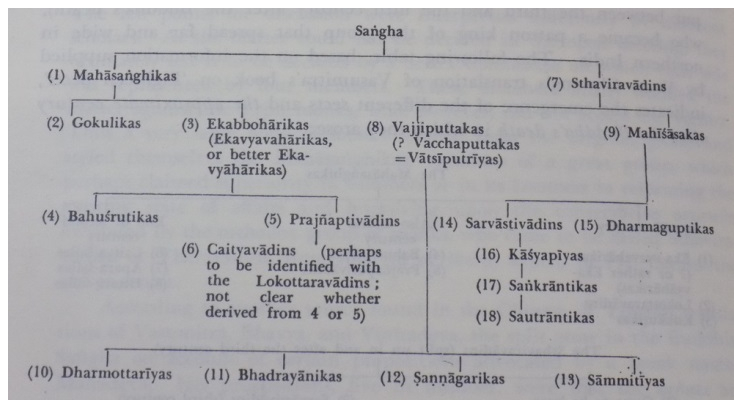
\includegraphics[scale=.35]{images/chap5-1.jpg}
\caption{Eighteen subgroups of the Buddhist \textit{saṅgha}}\label{chap5-fig1}
\end{figure}

The Buddha’s teachings emphasized the four noble truths and the eight-fold path; he called this the ‘Middle-Path’ as it “avoided the extremes of self-indulgence and self-mortification.” However, he was averse to metaphysical speculation, such as the origin and end of the universe; and left ten such questions unanswered (Bapat\index{Bapat, P. V.} 2001: 462-463). Among the six classical \textit{avaidika}\index{avaidika/nastika@\textit{avaidika/nāstika}} (heterodox) philosophies, four that are in the name of Buddhism viz. — \textit{Sautrāntika, Vaibhāṣika,\index{Vaibhasika@\textit{Vaibhāṣika}} Yogācāra}\index{Yogacara@\textit{Yogācāra}}\index{Sautrantika@Sautrāntika} and \textit{Mādhyamika}\index{Madhyamika@Mādhyamika} — have developed over time (\textit{infra}). The first two philosophies are said to belong to \textit{Hīnayāna}\index{Hinayana@Hīnayāna} or \textit{Theravāda}\index{Theravada@Theravāda} sect while the latter two to \textit{Mahāyāna}\index{Mahayana@Mahāyāna} sect. (Swami Satprakashananda\index{Satprakashananda, Swami} 2005: 68n) The details of the eighteen sub-groups of the Buddhist \textit{saṅgha} along with the above philosophies are discussed in detail in (Bapat 2001: 462-486). Hiriyanna\index{Hiriyanna, M.} says “while \textit{Hīnayāna} was atheistic and considered the Buddha\index{Buddha, the} as essentially a human being, though divinely gifted, the \textit{Mahāyāna} came to gradually deify him and adopted devout worship of him as a means to salvation... considerably influenced by theistic Hinduism.” (Hiriyanna 1948: 83).

\subsection*{2.1 Divergence from Hinduism}

Although the further sections of the paper seek to point out the proximity between Hinduism and Buddhism,\index{Buddhism} there are a few differences between Hinduism and Buddhism as pointed out by Hiriyanna, which are worth mentioning here. Firstly, while the Upaniṣadic doctrine was meant for a select few (i.e., not preached to all freely), “the characteristic feature of Buddhism was that it admitted no esoteric truths and was meant for all who were not satisfied with leading a life of natural inclinations.... Its message was for the plain man, and gave a general uplift of great significance.” Secondly, “while Brahmanism relied overmuch on the instruction given by others, Buddhism laid particular stress on self-reliance and self-effort in knowing the ultimate truth.” “For the rest, Buddhism was the same as Brahmanism... and believed in the same cosmological and eschatological views, including the doctrine of karma\index{karma@\textit{karma}}\index{Law of Karma}\endnote{ However, the \textit{vaidika}-s question the Buddhists about the basis of their belief in the doctrine of \textit{karma}\index{karma@\textit{karma}}\index{Law of Karma} when they reject the authority of the Veda.}.” (Hiriyanna 1948: 73)

\newpage

\subsection*{2.2 Limitation of Buddhism}

Mookerjee notes that —

\begin{myquote}
“The Buddha\index{Buddha, the} was skeptical of the ceremonial part of the Vedic religion as the vehicle of salvation. This is also endorsed by the Upaniṣad--s and the Bhagavadgītā.\index{Bhagavadgita@\textit{Bhagavadgītā}} But in the latter, we find a reconciliation between the practical life of the average man and the theoretical and contemplative life of the spiritual aspirant. The Vedic duties, which are obligatory and do not hold out any prospect of personal advantage, are to be observed as categorical imperatives. This subordination of personal ambition to impersonal duty is asserted to be an instrument of mental purification, which is the condition precedent of the emergence of inquisitiveness regarding the question of ultimate Truth and Destiny. This synthetic approach is absent in Buddhism.”\index{Buddhism} 

~\hfill (Mookerjee 2001: 597)
\end{myquote}

Further, Mookerjee says that —

\begin{myquote}
“It is a sad commentary on Buddhism as a religion and the separatist tendencies of its adherents that Sindhi monks had supported the Arab invaders and helped them in extirpating the Brāhmaṇa\index{brahmana@\textit{brāhmaṇa}} dynasty in Sind as early as 712 CE. It is also a surprise that the Buddhists committed to wholesale conversion whereas the Hindus survived this onslaught and preserved their ancestral faith... This facile changeover to an alien faith underlines the inherent weakness of the hold of Buddhism on the masses.” 

~\hfill (Mookerjee\index{Mookerjee, Satkari} 2001: 596)
\end{myquote}



\section*{3. Pollock’s\index{Pollock, Sheldon} Views and Responses}

While Max Müller\index{Müller, Max} states unequivocally that the entire faculties of (ancient) Indians were devoted to the ‘inward life of the soul’ to the exclusion of politics [§1]; Pollock seems to be hell bent on establishing the connection between culture, Sanskrit, \textit{kāvya},\index{kavya@\textit{kāvya}} grammar etc. on the one hand and political power on the other; most likely, this is inspired by Gruen’s thesis on the connection between the hegemony of the Roman empire and Latin literature\endnote{ Gruen (1990: 79-123). However, Malhotra\index{Malhotra, Rajiv} (2016) points out that there are more differences between Roman and Indian cultures than similarities, so such parallels need not necessarily be true.}. Presented in the rest of this section is an examination of the views of Pollock in the context of Buddhism, which he arrives at using his lens of ‘political philology’.

\newpage

\subsection*{3.1 Axial Theory}\index{Axial Theory}

Wittrock\index{Wittrock, Bjorn} summarizes Jaspers’\index{Jaspers, Karl} formulation of an Axial theory thus —

\begin{myquote}
“Jaspers believed that the distinctive feature in the emergence of human history... is the manifestation of a specific capacity —... the capacity of human beings to reflect upon and to give expression to an image of the world as having the potential of being different from what it was perceived to be here and now. The emergence of such images of the world, based on critical reflection, marked... the transition from \textit{Mythos} to \textit{Logos}, a breakthrough in critical reflexivity and, indeed, the emergence of history in the sense of the epoch in human existence characterized by a reflexive, historical consciousness. He termed this period the Axial Age. In temporal terms he located it in the centuries around the middle of the first millennium BCE.” 

~\hfill (Wittrock 2005: 62)
\end{myquote}

While Pollock\index{Pollock, Sheldon} disputes spatial causality and temporal locality of this “axial” age, he completely endorses the above summary and says “...under this description, there can be no doubt that “axial” moments exist at various times in history, and that Buddhist thinkers produced one such moment in early South Asia, effecting as they did a fundamental conceptual revolution in each of the three domains...” namely — reflexivity, historicity, and agentiality. (Pollock 2005: 398) Further he says

\begin{myquote}
“Jaspers asserted that one feature of the Axial Age is a new socio-political formation consisting in “the genesis of peoples who feel themselves a unity with a common language, a common culture, and a common body of myths.” But were we to accept this characterization, we would have to conclude that nothing like an Axial Age occurred, in India at least, prior to the twentieth century.” 

~\hfill (Pollock 2005: 399)
\end{myquote}

Although Pollock speaks of Sanskrit literary culture being spread from Afghanistan to Java and accepts the emergence of trans-local empires in India, he denies that a cultural unity emerged at that time. Quite on the contrary, Mookerji (2003:1-148) and Panikkar\index{Panikkar, K. M.} (1958:5-15) have argued that the cultural unity of India was firmly established irrespective (or in spite) of the political unity (of trans-local empires) of India. Hence it is clear from the above that Pollock is carefully cherry-picking only those features of the axial age asserted by Jaspers that is convenient to fit his theory, while ignoring other features which can be easily established. In addition, Pollock completely omits any discussion of the epistemological basis for “reflexivity” (where the world has the potential of being different from how it is perceived here and now)! Such omissions and misfits are extremely dangerous given that Pollock\index{Pollock, Sheldon} says that his “studying them is meant as a form of ‘actionable history’, an attempt to produce statements about past events that can inform the conduct of present practices,” quoting Bennett. (Pollock 2005: 400)


\subsection*{3.2 Buddhism as Axial Moment}\index{Buddhism}\index{Axial Theory}

Pollock notes the difference of opinion about the axial moment in India with Eisenstadt\index{Eisenstadt, S. N.} categorizing Buddhism as a “secondary breakthrough” while assessing late Vedic thought as wholly “axial”; and Jan Heesterman\index{Heesterman, Jan} arguing that it was the “gap” between Vedic revelation and ritual routinization that constituted India’s “axial turning point,” but gravitates to the following

\begin{myquote}
“sociality of early Buddhism that led to the institutionalization of the “transcendental breakthrough”..., singling out three aspects in particular: the “republic”-like religious assembly (that is, the \textit{saṅgha}); the democratizing promulgation of doctrine; and the development of a lay community of co-religionists (\textit{upāsaka}).” 

~\hfill (Pollock 2005: 401)
\end{myquote}

Quite on the contrary, Aiyaswamy Sastri\index{Sastri, Aiyaswami} states the common features of the \textit{Śramaṇa}\index{Sramana@\textit{Śramaṇa}} sects such as \textit{Aṇuvādin}-s, \textit{Ājīvika}-s,\index{Ajivika@Ājīvika} Jainism\index{Jainism} (all of which pre-date Buddhism), and Buddhism itself as:

\begin{enumerate}
\itemsep=0pt
\item “They challenged the authority of the Vedas.

 \item They admitted into their Church all members of the community irrespective of... \textit{varṇa}\index{varna@\textit{varṇa}} and \textit{āśrama}.

 \item They observed a set of ethical principles.

 \item They practiced a detached life with a view to liberating themselves...

 \item They could take to a life of renunciation any time after passing over the minor age.”

\end{enumerate}

\vspace{-.6cm}

\begin{flushright}
(Sastri 2001: 389-390)
\end{flushright}

essentially pointing out that these features of Buddhism were not breakthroughs achieved by Bud dhists themselves as claimed by Pollock. Furthermore, Vasudeva Sarana Agrawala\index{Agrawala, V. S.} points out that Pāṇini\index{Panini@Pāṇini} talks about a political republic (\textit{gaṇādhīna}) and the religious \textit{saṅgha} (\textit{nikāya}) in addition to monarchy (\textit{ekādhīna}) (Agrawala 1953: 424-427). Pāṇini also mentions the word “\textit{śramaṇa}”\index{Sramana@\textit{Śramaṇa}} (\textit{Astadhyayi}\index{Astadhyayi@\textit{Aṣṭādhyāyī}} 2.1.70) indicating the antiquity (pre-dating Buddha)\index{Buddha, the} of the word and therefore the sects going under that name. [see end of §1]

In addition, the \textit{Uttaramīmāmṣā-sūtra}-s\index{Uttaramimamsasutra@\textit{Uttaramīmāmṣā-sūtra-s}} point out that while the \textit{śūdra}-s\index{sudra@\textit{śūdra}}\break are excluded from undertaking the study of the Veda--s, they have the \textit{adhikāra}\index{adhikara@\textit{adhikāra}} to receive teachings in matters concerning the Vedānta (1.3.34-38). Śaṅkarācārya\index{Sankara@Śaṅkarā} affirms this, citing the example of Vidura and Dharmavyādha, and proclaims in his commentary that \textit{śūdra}-s too have \textit{adhikāra} for \textit{mokṣa}\index{moksa@\textit{mokṣa}} at least via the \textit{Itihāsa}-s\index{itihasa@\textit{itihāsa}} and \textit{Purāṇa}-s,\index{purana@\textit{purāṇa}} if not directly via the Vedic recitations and rituals (Apte\index{Apte, V. M.} 1960: 207-212). This is consistent with the tradition which holds that the Vedic vision must be communicated through the \textit{Itihāsa}-s and \textit{Purāṇa}-s (\textit{itihāsa-purāṇābhyāṁ vedaṁ samupabṛṁhayet}).

Hence, it is clear that the aspects of the \textit{saṅgha}, \textit{upāsaka}-community and the democratizing promulgation of doctrine was not any breakthrough achieved by the Buddha or Buddhists – as claimed by Pollock,\index{Pollock, Sheldon} but were the practices already in vogue that were followed.


\subsection*{3.3 Authorlessness of the Veda}

Pollock says:

\begin{myquote}
“While there can be hardly any doubt that the principal thrust of the Buddhist critique was directed toward actually-existing elements of the thought-world of early Brahmanism, it also seems likely that... its foundational principles, may have first been conceptualized as a defensive, even anti-axial,\index{Axial Theory} reaction to Buddhism\index{Buddhism}.... It is self-evident that no one would elaborate propositions of the sort we find Mīmāṁsā\index{Mimamsa@Mīmāṁsā} to have elaborated, such as the thesis of the authorlessness of the Veda, unless the authority of the Veda and its putative authors had first been seriously challenged.” 

~\hfill (Pollock 2005: 402)
\end{myquote}

The word \textit{Mīmāṁsā} means “the reasoning which has to be adopted to understand the connotation of a word or a sentence.” (Tarkabhushan\index{Tarkabhushan, Pramathanath} 2001: 160) It is true that Pūrvamīmāṁsā as a \textit{darśana}\index{darsana@\textit{darśana}} has its own idiosyncrasies such as the claims that

\begin{enumerate}
\itemsep=0pt
\item the universe was never created nor will it ever be destroyed (“it has existed as it is from eternity”) (Tarkabhushan\index{Tarkabhushan, Pramathanath} 2001: 164); and

 \item \textit{anupalabdhi}\index{anupalabdhi@\textit{anupalabdhi}} (non-perception) is a valid \textit{pramāṇa} (Svāmī Paramānanda Bhāratī\index{Svami Paramananda Bharati@Svāmī Paramānanda Bhāratī} 2014: 24-26).

\end{enumerate}

Pollock\index{Pollock, Sheldon} extracts the two features of ‘authorlessness’ and ‘ahistoricity’ of Veda discussed above based on the \textit{Pūrvamīmāṁsa-sūtra}-s\index{Mimamsasutra@\textit{Mīmāṁsasūtra}} 1.1.29-31 (Pollock 1989: 608). But the truth is that the \textit{Pūrvamīmāṁsa-sūtra}-s\break were composed by Jaimini\index{Jaimini} long before the advent of the Buddha,\index{Buddha, the} and hence the statement that these features of (\textit{Pūrva}-) \textit{Mīmāṁsā }\index{Purvamimamsasutra@\textit{Pūrvamīmāṁsā-sutra-s}}\index{Mimamsa@Mīmāṁsā}are a reaction to the Buddhist critique does not hold water [see end of §1]. And quite on the contrary, as Hiriyanna\index{Hiriyanna, M.} notes “it is Buddhism\index{Buddhism} which began as a ‘religion’ and it was forced, not long after, to become a ‘philosophy’ since it had to defend itself against the metaphysical schools of Hindu and Jaina\index{Jaina} thought.” (Hiriyanna 1948: 72).

While Pollock claims that (\textit{Pūrva})-\textit{Mīmāṁsā} holds the Veda to be authorless, the actual word used in (\textit{Pūrva})-\textit{Mīmāṁsā} is \textit{apauruṣeya};\index{apauruseya@\textit{apauruṣeya}} i.e., the assertion is that the Veda is self-revealed. This is but a natural consequence of the (\textit{Pūrva})-\textit{Mīmāṁsā} paradigm which does not accept \textit{nirguṇa Brahman}\index{Brahman@\textit{Brahman}} or \textit{Īśvara} and the idea that the universe was created. However, \textit{Nyāya-darśana}\index{Nyaya@Nyāya} does not accept this position and holds the Veda to be of divine origin (Tarkabhushan 2001: 152-156). Therefore, Pollock’s postulate that “a set of notions developed by Mīmāṁsā... may be said to have sought to deny the category of history altogether as irrelevant, or even antithetical, to real knowledge” (Pollock 1989: 607) need not be true, since it cannot be said that only the \textit{Pūrva-Mīmāṁsā} position held sway over all intellectuals of ancient/pre-modern India; especially when the \textit{Bṛhadāraṇyakopaniṣad} (2.4.10) itself proclaims that “the Vedas came into existence along with the creation from the Paramātman,\index{paramatman@\textit{paramātman}} the Supreme Creator as naturally as exhalation of a human being.” (Svāmī Paramānanda Bhāratī 2014: 22)

From an epistemological consideration, an interesting caveat may be observed here – just as the organs of perception — eyes, ears, nose, tongue, skin (\textit{pratyakṣa pramāṇa}\index{pratyaksa@\textit{pratyakṣa}}) and the law underlying inference/logic — are not man-made, similarly the Veda being a \textit{pramāṇa} is also not man-made. Therefore, we can assert that any \textit{pramāṇa} cannot be man-made; but man at best can invent extensions to these pramāṇa-s such as telescopes, spectacles, hearing-aids etc\endnote{ This understanding is thanks to Dr. Rama Phaniraj.}.

\vspace{-.3cm}

\subsubsection*{3.3.1 Ahistoricity}

Pollock extends his earlier argument about the authorlessness of the Veda and continues —

\begin{myquote}
“The Vedic corpus increasingly sought to escape confinement in any spatiotemporal framework,... Vedic texts are \textit{apauruṣeya}, produced by no author human or divine, and existing outside of all history whether cosmic or terrestrial. Buddhist holy texts, on the other hand, typically specify the place, time, audience, and of course speaker—the Buddha\index{Buddha, the}—thereby enmeshing the very truth of the message in its concrete historicity.” 

~\hfill (Pollock\index{Pollock, Sheldon} 2005: 409)
\end{myquote}

Firstly, as discussed in §3.3, \textit{apauruṣeya}\index{apauruseya@\textit{apauruṣeya}} need not mean the negation of divine origin of Veda according to \textit{darśana}-s\index{darsana@\textit{darśana}}. Tradition holds the Vedic statements as timeless truths. For example, although Newton came at a certain point in history and lived in a certain place, his discovery — the law of gravitation — is not subject to any spatiotemporal confinement\endnote{It may be the case that Newton’s formula of the force of attraction between two masses $m_1$ and $m_2$ separated by distance $r$ given by $F = G m_1 m_2/r^2$ might need correction in some cases, but the fundamental existence of the force of gravitation itself is unnegatable.}.~Hence, one view about the Veda--s is that the \textit{ṛṣi}-s to whom the \textit{mantra}-s were revealed do come in history, but the \textit{mantra}-s themselves are beyond time. Agrawala\index{Agrawala, V. S.} points out (through Kātyāyana’s\index{Katyayana@Kātyāyana} \textit{vārttika} on Pāṇini\index{Panini@Pāṇini} \textit{sūtra }4.3.105) that either Yājñavalkya\index{Yajnavalkya@Yājñavalkya} appears later in time or certain portions of the \textit{Śatapatha Brāhmaṇa }\index{Satapatha Brahmana@\textit{Śatapatha Brāhmaṇa}}attributed to Yājñavalkya were revealed later. (Agrawala 1953: 329-332) Also, there are studies on the \textit{Ṛgveda}\index{Rgveda@\textit{Ṛgveda}} from a historical angle by (Talageri\index{Talageri, Shrikant G.} 2000), for example.

The \textit{Tipiṭaka}-s\index{Tipitaka@\textit{Tipiṭaka}} got their final written form only after about two or three centuries after the \textit{nirvāṇa }\index{nirvana@\textit{nirvāṇa}} of the Buddha; and till that time, the Buddha’s teachings were transmitted orally [see §2]. Hiriyanna\index{Hiriyanna, M.} opines that the Buddhist canonical literature “may contain much that was actually uttered by Buddha; but there is no means of knowing for certain what those portions are” (Hiriyanna 1948: 72), especially in the light of divergent, if not contradictory, philosophies — ranging all the way from realism (\textit{sarvāsti-vāda}) to idealism (\textit{vijñāna-vāda}\index{vijnana@\textit{vijñāna}}) to nihilism\index{Nihilism} (\textit{śūnya-vāda}) — going under the name of Buddhism.\index{Buddhism}

In summary, the difference between Buddhism\index{Buddhism} and Vedic religion is not as pronounced as Pollock is suggesting here. 


\subsection*{3.4 Agentiality}

Pollock says

\begin{myquote}
“If Mīmāṁsā,\index{Mimamsa@Mīmāṁsā} the theory of the Veda, is about anything it is about the nature of deontic language, the obligation to act that the Veda places upon members of the vaidika community, the resolve (\textit{saṁkalpa}) one must make to act, and so on. But as Mīmāṁsā itself is very careful to explain—and indeed, is very rational when explaining—the truth-value of such paradigmatic Vedic commandments as “He who desires heaven must sacrifice” derives directly from the fact that their substance \textit{exceeds} the rational, instrumental understanding—precisely the understanding that underpins any authentic form of agentiality. The Veda’s injunction to act is meaningful precisely because it enunciates something that transcends the phenomenal, something inaccessible to observation, inference, or other form of empirical reasoning—something, in fact, irrational.”
\end{myquote}

and continues in the footnote as

\begin{myquote}
“Or, as the equally rationalistic Tertullian would have put it, \textit{credibile quia ineptum est}\endnote{ “\textit{Prorsus credibile est, quia ineptum est}” can be translated: “it is by all means to be believed, because it is absurd”. The context is a defence of the tenets of orthodox Christianity\index{Christianity} against docetism:” The Son of God was crucified: there is no shame, because it is shameful. And the Son of God died: it is by all means to be believed, because it is absurd. And, buried, He rose again: it is certain, because impossible.” — (De Carne Christi 5·4) (Connor 2014: 140)}: It is reason that dictates belief in a thing in direct proportion to the thing’s improbability.” 

~\hfill (Pollock\index{Pollock, Sheldon} 2006: 405-406)\textit{(italics as in the original)}
\end{myquote}


\subsubsection*{3.4.1 Irrationality}

Pollock essentially means that something that is inaccessible to observation, inference etc. is irrational, but {Mīmāṁsā} explains it very rationally; Pollock also draws parallel from Tertullian rationale\endnote{ This actually follows from Aristotlean logic, about which Robinson says “The scenario Aristotle is imagining is one in which there is an incredibly unlikely event in the past that the rhetor wants or needs to claim actually happened; to that end the rhetoric should invoke its very improbability (unlikelihood, incredibility) as an argument in favor of the story’s accuracy, its truthiness.” Robinson (2016: 236).} that “it is by all means to be believed, because it is absurd” which he undertook to demonstrate that the flesh of Christ was real. (Sider 1980) It is to be noted that the inaccessibility of Christ’s body a couple of centuries after he “died” or “ascended to heaven” is very much different from the inaccessibility of the subject matter to perception and inference here and now; and therefore such a parallel is untenable. More importantly, the tradition very clearly expounds that although perception, inference etc. have no access to the subject matter of Veda, the Vedic statements cannot contradict perception, inference etc.; therefore, the Veda is said to be supraational. In other words, correct understanding is that in which all apparent contradictions between \textit{śruti}\index{sruti@\textit{śruti}} (Veda), \textit{yukti }\index{yukti@\textit{yukti}}(logic/inference) and \textit{anubhava}\index{anubhava@\textit{anubhava}} (common universal experience) are resolved\endnote{ A common example given for the sake of understanding is — we see the Sun rising and setting everyday, but science says the Sun is stationary in the solar system; and we understand through the help of science that it is the rotation of the Earth which makes the Sun appear to rise in the East and set in the West.}. A famous dictum current in the tradition is “\textit{anubhava-anusārī śrutiḥ, śrutyanusārī yuktiḥ}.”\endnote{ As the \textit{śruti}\index{sruti@\textit{śruti}} is in line with \textit{anubhava}\index{anubhava@\textit{anubhava}} (everybody’s common experience), so should \textit{yukti}\index{yukti@\textit{yukti}} (logic) be in line with \textit{śruti}.}

Uttaramīmāṁsā\index{Uttaramimamsa@Uttaramīmāṁsā} has noted the limitation of \textit{tarka}\index{tarka@\textit{tarka}} (logic) and explicitly stated “\textit{tarkāpratiṣṭhānāt}...” (\textit{Brahma Sūtra} 2.1.11); that logic can only be as good as the data available, if not worse. Hence, the knowledge gained through \textit{anumāna}\index{anumana@\textit{anumāna}} must be verified through \textit{pratyakṣa}\index{pratyaksa@\textit{pratyakṣa}} (Svāmī Paramānanda\index{Svami Paramananda Bharati@\textit{Svāmī Paramānanda Bhāratī}} Bhāratī 2014: 20) and knowledge gained through \textit{śabda}\index{sabda@\textit{śabda}} must be verified through \textit{anubhava} to be doubt-free\endnote{ It might be argued that the existence of other \textit{loka}-s and cannot be verified by experience; but if one’s daily experience of different time-space realms in waking and dream, in deep-sleep, and the continuity of the individual’s existence across the three states is analyzed carefully, one cannot reject the possibility of other \textit{loka}-s and \textit{punar-janman}.}.


\subsubsection*{3.4.2 Deontic Language}

Pollock\index{Pollock, Sheldon} talks about “the obligation to act that the Veda places upon members of the \textit{vaidika} community” and a Vedic commandment “He who desires heaven must sacrifice” above reference in successive statements, perhaps without noticing the apparent contradiction between the two phrases. It is self-evident here that the desire to attain heaven is the driving force behind the sacrifice and not the Vedic commandment. The Veda never commands anyone to have desire, but only reveals the connection between a \textit{yajña}\index{yajna@\textit{yajña}} and its result. Hence, it is a gross misunderstanding to say that the Veda places obligation to act upon \textit{vaidika}-s.

The Veda enjoins \textit{nitya-naimittika-karman}-s\index{karma@\textit{karma}}\index{nityanaimittikakarman@\textit{nitya-naimittika-karman}} which do not seemingly produce any tangible result, but they prepare the mind of the performer for inquiry into the ultimate reality; and therefore it follows that a person desirous of undertaking such an inquiry must take to \textit{nitya-naimittika-karma}-s as a preparatory step [see §2.2].


\subsubsection*{3.4.3 Bourdieuean Doxa of \textit{Vaidika} World}

Pollock says that “The \textit{vaidika} world seems to have been one of pure Bourdieuean doxa, where both the order of society and one’s place in it went without saying, and where accordingly the possibility of reordering society and self... was outside the conceptual scheme. (Even renouncing society and self was routinized as normative.)” (Pollock 2005: 406)

There cannot be anything farther from the truth than this. Altekar points out that the different classes of Vedic society was not the rigid hereditary caste system — “The \textit{Śatapatha Brāhmaṇa}\index{Satapatha Brahmana@\textit{Śatapatha Brāhmaṇa}} [X·4·1·10] describes how some of the sons of Syāparṇa Sāyakāyana became \textit{Brāhmaṇa}-s, some \textit{Kṣatriya}-s\index{ksatriya@\textit{kṣatriya}} and some \textit{Vaiśya}-s\index{vaisya@\textit{vaiśya}}. Priests often accompanied their patron kings to the battlefield... and \textit{Kṣatriya}-s often sacrificed for others...” He further notes that the entire third \textit{maṇḍala} of the \textit{Ṛgveda}\index{Rgveda@\textit{Ṛgveda}} is ascribed to Viśvāmitra\index{Visvamitra@Viśvāmitra} (who is said to be both a Ṛṣi and a king); and that the Brāhmaṇa--s\index{brahmana@\textit{brāhmaṇa}} Gārgya\index{Gargya Balaki@Gārgya Bālāki} Bālāki and Gautama are taught about the nature of Brahman\index{Brahman@\textit{Brahman}} by the Kings Ajātaśatru\index{Ajatasatru@Ajātaśatru} and Pravāhaṇa\index{Pravahana Jaivali@Pravāhaṇa Jaivali} Jaivali respectively as spoken of in the \textit{Bṛhadāraṇyaka}\index{Brhadaranyaka Upanisad@\textit{Bṛhadāraṇyaka Upaniṣad}} [2·1] and \textit{Chāndogya}\index{Chandogya Upanisad@\textit{Chāndogya Upaniṣad}} [5·3] Upaniṣad--s. Thereby, the Buddha\index{Buddha, the} and the Mahāvīra\index{Mahavira@Mahāvīra} were not the only \textit{Kṣatriya}-s to teach philosophy. (Altekar\index{Altekar, K. S.} 2001: 226).

In the Vedic vision, true renunciation is born out of clear understanding and taking \textit{saṁnyāsa}\index{samnyasa@\textit{saṁnyāsa}} ceremoniously is but a symbolic, preparatory step; which was no doubt viewed as a ritual.


\subsection*{3.5 Semantic appropriation and Transvaluation}\index{transvaluation}

\subsubsection*{3.5.1 Sacrifice}

Pollock\index{Pollock, Sheldon} points out that

\begin{myquote}
“In the Kuṭadanta Sutta, for example, a Brāhmaṇa is dissuaded from his original intention to offer a blood sacrifice... by the tale of a far more successful sacrifice where neither were any oxen slain, neither goats, nor fowls, nor fatted pigs, nor were any kinds of living creatures put to death.... But even this kind of sacrifice—where we can observe how non-violence is coupled with non-coercion... entrance into the Buddhist order, and Buddhist forms of meditation.” 

~\hfill (Pollock 2006: 402-403)
\end{myquote}

While it may be true that certain Vedic rites might include animal sacrifices of a “cruel, horrible and revolting” nature; many non-violent “sacrifices” or \textit{Jñāna-yajña}-s\index{yajna@\textit{yajña}} are also present in the Veda-s; for example — The \textit{Mahānārāyaṇa Upaniṣad}\index{Mahanarayana Upanisad@\textit{Mahānārāyaṇa Upaniṣad}} (80th \textit{anuvāka}) talks of a ``\textit{yajña} in which \textit{śraddhā}\index{sraddha@\textit{śraddhā}} (faith) is the performer’s wife, his body is firewood, his breast is the shrine”, (Bhattacharya 2001: 559) \textit{kāma }(desire) is ghee, \textit{manyu} (anger) is the animal to be sacrificed etc. The \textit{Bhagavadgītā}\index{Bhagavadgita@\textit{Bhagavadgītā}} (2.45) too talks of many other \textit{yajña}-s such as \textit{tapo-yajña}, \textit{yoga-yajña}, \textit{dhyāna-yajña}, \textit{japa-yajña}\index{yajna@\textit{yajña}} etc., and in more places than one suggests their superiority over mere \textit{dravya-yajña} in progressing towards attaining the ultimate end of \textit{mokṣa}\index{moksa@\textit{mokṣa}} (salvation). [see §2.2]

Hiriyanna also says that —

\begin{myquote}
“The (Buddhist) canonical literature, no doubt, now and again criticizes Brahmanism, but mostly on its ritualistic side.... An important consequence of this rejection of ritual was the emphasis placed on morality which, though by no means ignored in Brahmanism, was somewhat assigned a subordinate place in it. The references to the Upaniṣadic doctrine, the other aspect of Brahmanism, are far fewer, showing that Buddhism\index{Buddhism} did not diverge from it very much.” 

~\hfill (Hiriyanna\index{Hiriyanna, M.} 1948: 72)
\end{myquote}

In a slightly different context, which is presented as an attack on the \textit{Puruṣasūkta}\index{Purusasukta@Puruṣasūkta} by the Buddha,\index{Buddha, the} Pollock\index{Pollock, Sheldon} says that “The sacrifice of the\break Puruṣa and the fixed social order that thereby emerged seem almost recombined in the Mīmāṁsā\index{Mimamsa@Mīmāṁsā} doctrine of the fixity of the right to sacrifice, \textit{adhikāra},\index{adhikara@\textit{adhikāra}} which was reserved to the three twice-born orders.”; as if to suggest that the presentation of sacrifice of the \textit{Puruṣa} leads to fixation of right to sacrifice to \textit{dvija}-s (twice-born) only and is therefore discriminating against some people by not allowing them to\break sacrifice. Pollock perhaps fails to notice, while coming up with his explanation on \textit{apauruṣeyatva} as authorlessness, that the \textit{Puruṣasūkta} itself says that “from the \textit{yajña} of \textit{Puruṣa}, the \textit{Ṛg}-, \textit{Sāma}\index{Samaveda@\textit{Sāmaveda}}- and \textit{Yajur-veda}-s\index{Yajurveda@\textit{Yajurveda}},\break and the Vedic meters (\textit{chandas}) were born”. [§3.3.1]

Swami Sharvananda presents the insight behind describing the creation of the cosmos as a \textit{yajña }thus —

\begin{myquote}
“the Vedic \textit{Ṛṣi}-s looked upon the entire cosmic process as the performance of a great sacrifice, and believed that man’s spiritual nature can best be quickened if he tried to mould himself in consonance with that cosmic order order.... In fact, this spirit of sacrifice, restraint, and harmony through love, and desire for the attainment of immortality in life came to be the dominant factors of the cultural life... The last \textit{sūkta} of the \textit{Ṛgveda}\index{Rgveda@\textit{Ṛgveda}} breathes this out unequivocally thus: Assemble together, speak with one voice,... United be the thoughts of all... may all happily reside.” 

~\hfill (Sharvananda 2001: 198)
\end{myquote}


\subsubsection*{3.5.2 Negation of \textit{Ātman}}\index{atman@\textit{ātman}}

Pollock says that

\begin{myquote}
“...positive inversions or transvaluations\index{transvaluation} in early Buddhism\index{Buddhism} of core \textit{vaidika} values are complemented by a range of pure negations; foremost among these is \textit{an-atta} (\textit{an-ātmā}), the denial of a personal essence whereby the fundamental conception of Upanishadic thought is canceled. All this evidence suggests that semantically Buddhism sought to turn the old \textit{vaidika} world upside down by the very levers offered by the \textit{vaidika} world.” 

~\hfill (Pollock\index{Pollock, Sheldon} 2006: 404)
\end{myquote}

Bhattacharya points out the reason for negation of \textit{ātmā} by the Buddha\index{Buddha, the} thus: “In order to root out desire (\textit{kāma}), attempts are made in the doctrine of the Buddha to show that there is neither the subject nor the object of desire, and if that be so, naturally desires can in no way arise.” On the other hand, the Upaniṣad--s say that “when a man understands both the subject (himself) and the object of desire as non-separate from Brahman\index{Brahman@\textit{Brahman}} (or Ātman), there can arise no desire (or fear, sorrow etc.)” (Bhattacharya 2001: 564-565) In other words, the Buddha seeks to deny the existence of both subject and object completely; while the Upaniṣad--s say that the subject and object borrow their existence from \textit{Brahman}, and thereby have no existence of their own, separate from \textit{Brahman}, and thus \textit{Brahman} alone exists. Hence, it is clear that both the Buddha and the Upaniṣad--s are seeking the same end, but there is a difference in the sense in which the word \textit{ātman} is used.

In addition, it is to be noted that the process of negation — \textit{neti}, \textit{neti} (not this, not this) — occurs verily in the Upaniṣad--s and \textit{Brahman} or \textit{Ātman} is proclaimed as the self-evident truth which can never be negated. It may be interesting to note in this context that Śankarācārya\index{Sankara@Śankarā} is accused of being a \textit{pracchanna-bauddha }(crypto-Buddhist); and while the Advaitic tradition does not accept this (Apte\index{Apte, V. M.} 1960: xxvii), it goes to speak of the proximity between Hinduism (especially Advaita\index{Advaita} Vedānta which rests on the three pillars of the Upaniṣad--s, the \textit{Uttara-mīmāṁsā-sūtra}-s and the \textit{Bhagavadgītā}\index{Bhagavadgita@\textit{Bhagavadgītā}}) and Buddhism. Hence, it seems here that Buddhism has much in common with the vision of the Upaniṣad--s and \textit{Gītā} than the differences which Pollock is trying to highlight.

\newpage

\subsection*{3.6 Media of Preaching Buddhism}

Pollock argues that, keeping the Mīmāṁsā\index{Mimamsa@Mīmāṁsā} theory of language in mind,

\begin{myquote}
“...the early Buddhists rejected the use of Sanskrit, the language of the gods, whether in favor of local dialects or Pali, a new hieratic competitor language. It is no small measure of the exhaustion of the Axial\index{Axial Theory} energies of early Buddhism\index{Buddhism} that around the beginning of the Common Era in the north at least this old opposition was abandoned and the repressed returned: Buddhists turned to Sanskrit with a vengeance, translating their canon into the language.” 

~\hfill (Pollock\index{Pollock, Sheldon} 2006: 409)
\end{myquote}

Upadhye points out that “Vedic literature does give some glimpses of popular speeches; but no literature in them has come down to us. Classical Sanskrit... respectfully shelved all that was obselete in the Vedic speech and studiously eschewed all that belonged to the popular tongue... Whenever a preacher or a prince wanted to address the wider public..., the tendency to employ a popular dialect of the day was but natural. That is how... Mahāvīra\index{Mahavira@Mahāvīra} and Buddha\index{Buddha, the} preferred to preach in the local Prakrits of eastern India,” similarly Aśoka\index{Asoka@Aśoka} and Khāravela\index{Kharavela@Khāravela} addressed their subjects in Prakrit. Again, he observes that the \textit{gāthā} literature of the Buddhists is a good specimen of queer admixture of Sanskrit and Prakrit, suggesting that was no conflict between the two. (Upadhye 2001: 164-165)

Pollock tries very hard to establish that early Buddhists rejected the use of Sanskrit due to the theory of language of the Mīmāṁsaka-s; and therefore the onus is on him to argue why the Buddhists later turned to Sanskrit. He forwards some arguments such as —

\begin{itemize}
\itemsep=0pt
\item Sanskrit is the language of learning

 \item syndrome of competition with Brahmanical communities for popular esteem

 \item technical precision of Sanskrit

 \item many \textit{Brāhmaṇa}-s\index{brahmana@\textit{brāhmaṇa}} such as Nāgārjuna\index{Nagarjuna@Nāgārjuna}, Nāgasena\index{Nagasena@Nāgasena} etc. converted to Buddhism,

\end{itemize}

and finding none of them satisfactory, only says in conclusion that at least Buddhists used Sanskrit for the first time to compose literature outside of the Veda--s. (Pollock 2006: 53-59)

Citing the \textit{Vinaya Piṭaka}, Bapat says that “the Buddha had permitted his followers to use their own speech for the purpose of instruction and preaching.” He further says that the \textit{Sarvāstivādin}-s adopted Sanskrit since people in the north-western part of India were conversant with the same; while the \textit{Mahāsaṅghika}-s\index{Mahasanghika@\textit{Mahāsaṅghika}} adopted Prakrit as the people in the eastern regions (Magadha and Aṅga) were familiar with the same (see Figure 1). (Bapat\index{Bapat, P. V.} 2001: 460-461) Hence, the choice of language for preaching seems to be very pragmatic, rather than due to sectarian (or religious) differences, or for the sake of rejection of an esoteric linguistic theory.

If by “literature outside of the Vedas”, Pollock\index{Pollock, Sheldon} means that literature which rejects the Vedic authority, or is critical of the Veda, then perhaps only non-adherents of Vedic religion can compose such literature. On the other hand, it if means that literature which does not necessarily have to criticize or reject the Veda, then there is abundant literature in Sanskrit pre-Buddha\index{Buddha, the} including the \textit{sūtra}-s of various \textit{darśana}-s\index{darsana@\textit{darśana}} — {Sāṅkhya},\index{Sankhya@Sāṅkhya} {Yoga}\index{Yoga}, {Pūrva-mīmāṁsā},\index{Mimamsa@Mīmāṁsā} {Uttaramīmāṁsā} etc. Agrawala\index{Agrawala, V. S.} says that “Pāṇini’s\index{Panini@Pāṇini} reference to Vāsudeva as an object of bhakti\index{bhakti@\textit{bhakti}} throws light on the antiquity of the bhakti cult,” hence at least the core portion of the \textit{Mahābhārata}\index{Mahabharata@\textit{Mahābhārata}} (or \textit{Jaya}) including the \textit{Bhagavadgītā}\index{Bhagavadgita@\textit{Bhagavadgītā}} was composed before the advent of Buddha.


\subsection*{3.7 Caste and Social Reform}

Pollock says that

\begin{myquote}
“Buddha explains the entirely contingent nature of all social categories, and the process of social evolution through which this contingency manifests itself. The Brahman\index{Brahman@\textit{Brahman}} is not superior biogenetically; indeed, “Brahman” is shown (by etymology) not even to be a natural kind, he is simply one who “keeps away from bad things,” as the true Śūdra\index{sudra@\textit{śūdra}} is anyone who “leads a cruel, mean life.” The target of this discourse is of course the discourse of the celebrated Rigvedic text, the \textit{Puruṣasūkta}\index{Purusasukta@Puruṣasūkta}...” 

~\hfill (Pollock 2006: 407)\textit{(spelling/italics as in the original)}
\end{myquote}

Nowhere do the Veda--s speak of a \textit{Brāhmaṇa} as biogenetically superior. It has been shown in §3.4.3 above that \textit{Brāhmaṇa}-s have been taught by \textit{Kṣatriya}-s\index{ksatriya@\textit{kṣatriya}}, and also, how the classes were fluid initially. Agrawala mentions that Pāṇini has a \textit{sūtra} describing the \textit{bhāva} (nature) and \textit{karma}\index{karma@\textit{karma}} (conduct) which should characterize a \textit{Brāhmaṇa}, and also speaks of a degraded \textit{Brāhmaṇa}\index{brāhmaṇa@\textit{brāhmaṇa}} as \textit{ku-brāhmaṇa} (Agrawala\index{Agrawala, V. S.} 1953: 74). Commenting on the Buddhist critique of the caste system, Mookerjee says

\begin{myquote}
“The Buddhists were hard critics of caste, particularly of the Brāhmaṇa caste and the hereditary privileges incidental to caste hierarchy.... It is however, a mistake, which has become a confirmed belief among the modern social reformers, to suppose that the Buddha\index{Buddha, the} was a social reformer. It is true that he stood against the Brāhmaṇa’s claim to superiority.... But he did nothing to interfere with the social organization of the time.... It is again, a superstition to presume that the Buddha was a democrat or an advocate of socio-political equality. He was a perfect stranger to these modern ideas, and the political ideal of a \textit{cakravartin} (emperor) ruling over the whole of India was dearest to his heart. So far as the Order was concerned, it was organized on the basis of equal rights subject to the abbot. And so long as he lived, he maintained his supremacy in the Church.” 

~\hfill (Mookerjee\index{Mookerjee, Satkari} 2001: 585-586)
\end{myquote}

One of the prominent social reformers of early 19th century, Swami Dayananda\index{Swami Dayananda Saraswati} Saraswati who established the Arya-Samaj, vowed his allegiance to the Veda--s and yet was critical of the caste system then practiced; which clearly shows that the vulgarized rigid hereditary caste system based on birth that was then practiced is not prescribed by the Veda--s (Gore 2011: 128).

Mukherjee notes that —

\begin{myquote}
“Continuity of the caste system in India, from ancient down to the modern times, is a grand riddle for the social and economic historians as well as the sociologists. Max Weber, the famous sociologists has tried to analyze social stagnation in India in terms of the metaphysical aspects of its caste-system. But the Indian caste-system has not been wholly influenced by religious or metaphysical considerations. It has several social or economic bases. One of the reasons of the continuity of the caste-system in modern India is thus the fact that it has permitted sufficient upward and lateral mobility withing the caste-system as a whole.” 

~\hfill (Mukherjee\index{Mukherjee, Sobhanlal} 2011: 611-613)
\end{myquote}


\subsection*{3.8 Conversion}

Pollock stresses voluntarism of early Buddhism\index{Buddhism} (and Jainism)\index{Jainism} through the idea of “\textit{śaraṇāgamana},\index{saranagamana@\textit{śaraṇāgamana}} taking refuge in the Buddha” or conversion, and says that although “historically exogenous communities were eventually incorporated in some measure in the \textit{vaidika} social sphere, nowhere and never did this process have an evangelical dimension.” (Pollock\index{Pollock, Sheldon} 2006: 406).

The \textit{vaidika} society has the \textit{saṁskāra}\index{samskara@\textit{saṁskāra}} of \textit{upanayana} from when the study of Veda--s is undertaken. For a \textit{vaidika}, the Veda-s is itself omniscient or are the words of an omniscient God; and therefore, he surrenders to the very words (of God). Only when such \textit{śraddha}\index{sraddha@\textit{śraddha}} is lacking will he seek any means outside of the Veda-s. In addition, there are a number of deities described in the Veda-s themselves, or in the later \textit{Purāṇa}-s\index{purana@\textit{purāṇa}} and \textit{Itihāsa}-s\index{itihasa@\textit{itihāsa}}, to whom one can surrender, and there are many choices from which to pick an \textit{iṣṭa-devatā}.\index{devata@\textit{devatā}} Or else, one can even surrender to one’s guru who is the guiding light in one’s life and spiritual progress. Hence, it does not seem correct to say that the voluntarism of Buddhism (or Jainism) alone is stressed through the idea of \textit{śaraṇāgamana}. However, as noted in §2.1 above, voluntarism perhaps might be taken as laying emphasis on self-effort to the negation of taking instruction from others, but the idea of \textit{śaraṇāgamana} (surrender) itself does not seem to gel well with the ideology of self-effort.

While talking about the spread of Buddhism, Swami Vivekananda\index{Swami Vivekananda}\break says —

\begin{myquote}
“I have every respect and veneration for Lord Buddha,\index{Buddha, the} but mark my words, the spread of Buddhism was less owing to the doctrines and the personality of the great preacher, than to the temples that were built, the idols that were erected, and the gorgeous ceremonials that were put before the nation. Thus Buddhism progressed. The little fire-places in the houses in which the people poured their libations were not strong enough to hold their own against these gorgeous temples and ceremonies; but later on the whole thing degenerated.” 

~\hfill (Vivekananda 2007: 132)
\end{myquote}

At this point, it is interesting to note what Max Müller\index{Müller, Max} has said about conversion and Buddhism —

\newpage

\begin{myquote}
“History seems to teach that the whole human race required a gradual education before, in the fulness of time, it could be admitted to the truths of Christianity. All the fallacies of human reason had to be exhausted, before the light of a higher truth could meet with ready acceptance.... That religion, the religion of Buddha,\index{Buddha, the} has spread, far beyond the limits of the Aryan world, and, to our limited vision, it may seem to have retarded the advent of Christianity among a large population of the human race. But in the sight of Him with whom a thousand years are but as one day, that religion, like all the ancient religions of the world, may have but served to prepare the way of Christ, by helping, through its very errors, to strengthen and to deepen the ineradicable yearning of the human heart after the truth of God.
\end{myquote}

\begin{myquote}
Though the religion of the Buddha be of all religions the most hostile to the old belief of the Brahmans, — the Buddhists standing to the Brahmans in about the same relation as the early Protestants to the Church of Rome, — yet the very bitterness of this opposition proves that Buddhism\index{Buddhism} is peculiarly Indian. Similar ideas to those proclaimed by Buddha were current long before his time, and traces of them may be found even in other countries.” 

~\hfill (Müller\index{Müller, Max} 1860: 32-33)
\end{myquote}

Max Müller, perhaps in a strange way, notes the proximity between Hinduism and Buddhism by comparing them with Roman Catholic and Protestant\index{Protestant Christianity} Christianity.\index{Christianity} It is not apparently clear if Max Müller has noticed the lack of the hold of Buddhism on the masses [as discussed in §2.2 above] and is therefore saying it prepares the way for conversion to Christianity; or he is simply asserting his supremacist attitude.

\vspace{-.3cm}

\section*{4. Decline of Buddhism in India \hfill\break and Recent Revival}

Mookerjee\index{Mookerjee, Satkari} (2001: 576) notes that “Buddhism, as preached by the sage of the Śākya clan and as it appears in the recorded versions of the Pali cannon, was not meant to be a full-fledged religion covering the entire gamut of human interests. The Buddha “claimed to have discovered a path to salvation from the evanescent, miserable existence in the world, and he preached this to all and sundry.... He left the nature of ultimate reality... an open question.” Further, he says that Buddhism’s progressive deviation from the ancient moorings increasing the number of gods and goddesses in the pantheon and rise in ritualism reduced its popularity among the intellectuals. While talking about \textit{bhakti}\index{bhakti@\textit{bhakti}} and the \textit{purāṇa}-s\index{purana@\textit{purāṇa}}, Swami Vivekananda says “we ought to be grateful to them [Purāṇa-s] as they gave us in the past a more comprehensive and better popular religion than what the degraded later-day Buddhism was leading us to.” (Vivekananda\index{Swami Vivekananda} 2007: 332). The decisive blow to Buddhism\index{Buddhism} most likely came from the destruction of monasteries and massacre of Buddhist monks at the hands of the Turks (Mookerjee\index{Mookerjee, Satkari} 2001: 579, 595). Although there are not too many adherents of Buddhism in India, yet the Buddha\index{Buddha, the} is very much revered nonetheless and also considered as an \textit{avatāra} of Viṣṇu. Also, some of the high points of Buddhism are assimilated into what is popularly known as Hinduism today, and Buddhism continues to live in that sense.

Fast forwarding to British India, Barua points out that \textit{Mahāyāna}\index{Mahayana@Mahāyāna} Buddhism being liberal in nature, had managed to survive in some pockets in the Himalayan regions and the Chittagong area, but a need was felt in the 18/19th centuries CE to revive the more conservative \textit{Theravāda}\index{Theravada@Theravāda} sect. During the same time frame, Dr. Ambedkar\index{Ambedkar, B. R.} was fighting for the cause of the depressed classes; and also demanded a separate electorate for the depressed classes. In a turn of events, when only reservations for the depressed classes were sanctioned; Dr. Ambedkar finally led his followers through mass conversion to \textit{Theravāda} Buddhism in 1956 at Nagpur. (Barua 2011: 708-709)

\vspace{-.3cm}

\section*{5. Conclusion}

The paper presents some of the views of Pollock\index{Pollock, Sheldon} about Buddhism being a sort of revolution against the prevailing Vedic religion and society. An analysis of the said views presented here shows that only those features of the axial\index{Axial Theory} age are carefully selected which can then be applied to another careful selection of features of a perceived conflict between Buddhism and the Vedic religion, between Sanskrit and Prakrit to present his preconceived notions as if they are the logical conclusion of some carefully well-examined arguments.

\vspace{-.3cm}

\section*{Bibliography}

\begin{thebibliography}{99}
\itemsep=1pt
\bibitem{chap5-key01} Agrawala, V. S. (1953). \textit{India as Known to Pāṇini}. Lucknow: University of Lucknow.

 \bibitem{chap5-key02} Altekar, K. S. (2001). “Vedic Society”. In Chatterji \textit{et al} (2001). pp. 221–233.

 \bibitem{chap5-key03} Apte, Vasudeo Mahadeo. (1960). \textit{Brahma-sūtra Śānkara-bhāṣya} translated into English. Bombay: Popular Book Depot.

 \bibitem{chap5-key04} Arnason, Johann P., Eisenstadt, S. N., and Wittrock, Björn. (Ed.s) (2005). \textit{Axial Civilizations and World History}. Leiden, Boston: Brill.

 \bibitem{chap5-key05} Banerjee, Anukul Kumar. (2001). “Buddhist Literature”. In Chatterji (2001). pp. 184–210.

 \bibitem{chap5-key06} Bapat, P. V. and Dutt, Nalinaksha. (2001). “Schools and Sects of Buddhism”. In Chatterji \textit{et al }(2001). pp. 456–502.

 \bibitem{chap5-key07} Barua, Dipak Kumar. (2011). “Buddhism and Jainism”. In Raychaudhury (2011). pp. 707–737.

 \bibitem{chap5-key08} Bhattacharya, Haridas (Ed.) (2001). \textit{The Cultural Heritage of India}, Volume III. Kolkata: The Ramakrishna Mission Institute of Culture.

 \bibitem{chap5-key09} Bhattacharya, Vidhushekhara. (2001). “Buddhism in Relation to Vedānta”. In Chatterji \textit{et al}. (2001). pp. 559–574.

 \bibitem{chap5-key10} Chatterji, Suniti Kumar. (Ed.) (2001). \textit{The Cultural Heritage of India}, Volume V. Kolkata: The Ramakrishna Mission Institute of Culture.

 \bibitem{chap5-key11} —. Dutt, Nalinaksha., Pusalker, A. D., and Bose, Nirmal Kumar. (Ed.s) (2001). \textit{The Cultural Heritage of India}, Volume I. Kolkata: The Ramakrishna Mission Institute of Culture.

 \bibitem{chap5-key12} Connor, Steven. (2014). \textit{Beckett, Modernism and the Material Imagination. }New York: Cambridge University Press.

 \bibitem{chap5-key13} Gore, M. S. (2011). “Social Reform Movements in Northern, Western and Southern India”. In Raychaudhury \textit{et al.} (2011). pp. 116–138.

 \bibitem{chap5-key14} Gruen, Erich S. (1990). \textit{Studies in Greek Culture and Roman Policy}. Berkeley: University of California Press.

 \bibitem{chap5-key15} Hiriyanna, M. (1948). \textit{Essentials of Indian Philosophy}. Reprint 2008. Delhi: Motilal Banarsidas.

 \bibitem{chap5-key16} Kamat, Suryanath U. (2015). \textit{A Concise History of Karnataka}. Bengaluru: M. C. C. Publications.

 \bibitem{chap5-key17} Malhotra, Rajiv. (2016). \textit{The Battle for Sanskrit}. Noida: Harper Collins.

 \bibitem{chap5-key18} Maṇi (2012). Mūlasūtrālu (Fundamentals)(In Telugu). Rajamaṇḍri: Maheśvara Image Graphics,

 \bibitem{chap5-key19} Mookerjee, Satkari. (2001). “Buddhism in Indian Life and Thought”. In Chatterji \textit{et al} (2001). pp. 575–600.

 \bibitem{chap5-key20} Mookerji, Radha Kumud. (2003). \textit{The Fundamental Unity of India}. Delhi: Bharatiya Vidya Bhavan.

 \bibitem{chap5-key21} Mukherjee, Sobhanlal. (2011). “Growing Urbanization in Modern India”. In Raychaudhury (2011). pp. 589–619.

 \bibitem{chap5-key22} Müller, Max. (1860). \textit{A History of Ancient Sanskrit Literature}. London: Williams and Norgate.

 \bibitem{chap5-key23} Panikkar, K. M. (1958). \textit{The Determining Periods of Indian History}. Delhi: Bharatiya Vidya Bhavan.

 \bibitem{chap5-key24} Pollock, Sheldon. (1989). “Mīmāṁsā and the Problem of History in Traditional India”. \textit{Journal of the American Oriental Society} 109.4, pp. 603–610.

 \bibitem{chap5-key25} —. (2005). “Axialism and Empire”. In Arnason et al. (2005). pp. 397–450.

 \bibitem{chap5-key26} —. (2006). \textit{The Language of Gods in the World of Men}. Berkeley: University of California Press.

 \bibitem{chap5-key26a} \textbf{\textit{Rājataraṅgiṇī}}. See Stein (1900).

 \bibitem{chap5-key27} Raychaudhury, Tapan., Bhattacharya, Sukumar., and Das Gupta, Uma. (Ed.s) (2011). \textit{The Cultural Heritage of India}. Volume VIII. Kolkata: The Ramakrishna Mission Institute of Culture.

 \bibitem{chap5-key28} Robinson, Douglas. (2016). \textit{The Deep Ecology of Rhetoric in Mencius and Aristotle: A Somatic }

 \bibitem{chap5-key29} \textit{ Guide. }New York: SUNY Press.

 \bibitem{chap5-key30} Sastri, Pandit N. Aiyaswami (2001). “Śramaṇa or Non-Brāhmaṇical Sects”. In Chatterji \textit{et al}. (2001). pp. 389–399.

 \bibitem{chap5-key31} Sider, Robert D. (1980). “Credo quia absurdum?”. \textit{Classical World} 73, pp. 417–419.

 \bibitem{chap5-key32} Sreedharan, E. (2004). \textit{A Textbook of Historiography: 500 BC to AD 2000}. New Delhi: Orient Longman Pvt. Ltd. ISBN: 9788125026570.

 \bibitem{chap5-key33} Stein, M. A. (1900). \textit{Kalhaṇa’s Rājatarangiṇī}. Westminster: Archibald Constable and Company, Ltd.

 \bibitem{chap5-key34} Svāmī Paramānanda Bhāratī. (2014). \textit{Vedānta Prabodha} (In Kannada). Bengaluru: Jñānasaṁvardhanī Pratiṣṭhānam.

 \bibitem{chap5-key35} Swami Satprakashananda. (2005). \textit{Methods of Knowledge according to Advaita Vedanta}. Kolkata: Advaita Ashrama.

 \bibitem{chap5-key36} Swami Sharvanada. (2001). “The Vedas and their Religious Teachings”. In Chatterji \textit{et al}. (2001). pp. 182–198.

 \bibitem{chap5-key37} Swami Vivekananda. (2007). \textit{Lectures from Colombo to Almora}. Kolkata: Advaita Ashrama.

 \bibitem{chap5-key38} Talageri, Shrikant G. (2000). \textit{The Rigveda: A Historical Analysis}. New Delhi: Aditya Prakashan.

 \bibitem{chap5-key39} Tarkabhushan, Pramathanath. (2001). “Pūrva-Mīmāṁsā”. In Bhattacharya (2001). pp. 151–167.

 \bibitem{chap5-key40} Upadhye, A. N. (2001). “Prakrit Language and Literature”. In Chatterji (2001). pp. 164–183.

 \bibitem{chap5-key41} Wittrock, Björn. (2005). “The Meaning of the Axial Age”. In Arnason \textit{et al} (2005). pp. 51–86.

 \end{thebibliography}

\theendnotes

\label{chapter5-end}
